\section{Where Earth hides in the models}

A model carries Earth wherever one of its values or forms agrees with Earth because Earth set it, and
such a part, run on the Moon, returns Earth's answer to a lunar question. Table~\ref{tab:inventory} lists
the instances found on the paths the lunar runs use, each with its form and its state at Terluna commit
186b294; the defect log in the accompanying repository adds those found off those paths and gives each
one's discovery, evidence, repair and measured effect. The inventory separates two kinds. In a limitation
the code does what it was written to do, on the world it was written for. In a defect the code is wrong on
its own terms, on every world. Four of the five forms are limitations; the fifth holds the released codes'
defects.

\textbf{Constants written into the code.} A dimensional constant carries the scale of the world it was
set on, and gravity is the commonest. CM1 release 22 sets it to 9.81~m\,s$^{-2}$ in four places on the
lunar cases' paths, its dynamics, the conversion of pressure to layer mass in its RRTMG radiation
\autocite{iacono2008radiative}, its CAPE diagnostic and the Morrison microphysics, and in several schemes
those cases leave unselected; Morrison's fall-speed laws $V = aD^b$ and their caps hold Earth's gravity in
their coefficients.\claim{H01} WRF-ELEC's NSSL scheme sets 9.8 twice and ties the ventilation of
evaporating rain and depositing ice to Earth's fall-speed coefficients.\claim{H02} Earth sets two thresholds
and a time step in WRF-ELEC's lightning. A breakdown field scaled with the air's density
\autocite{dwyer2003fundamental} and capped at 180~kV\,m$^{-1}$ acts on Earth only below about 4.5~km,
beneath where flashes start, and in lunar air below about 36~km, where it lowers the field by 44\% at the
ground. A ground strike is declared when a channel reaches air warmer than $-7$\,\textdegree C, about 5~km
above Earth's ground and 27--34~km above the Moon's. A 0.75~s sub-step is sized for 500~m layers and
Earth's fall speeds.\claim{H03} Earth's seas set SWAN's constants. It reduces its linear wind input above a
knee fixed at 1~Hz, a value its source comments call largely arbitrary, and the fixed knee breaks the
model's gravity similarity: stock SWAN misses a sixfold similarity test by
5.44\% in significant wave height.\claim{H04} It also fixes the air's density at 1.28~kg\,m$^{-3}$, where the air over the lunar seas
holds about 1.40.\claim{H05} Earth's composition and rotation complete the set: RRTMG takes carbon dioxide
from the calendar year and carries Earth's methane, nitrous oxide, halocarbons and ozone, and CM1's beta
plane derives its gradient from Earth's rotation and a 6,370~km radius.\claim{H06} Each constant is right
for Earth, and can be made right for the Moon as far as its lunar value is known.

\textbf{Units of time.} A formula written per day, and a process that matters only over a long run, both
hold Earth's calendar. Slingo's convective cover in PlaSim, $0.245 + 0.125\ln P$ in the form PlaSim's
manual gives it \autocite{slingo1991response,lunkeit2012plasim}, with $P$ the convective rain in
millimetres per day, converts the model's rain to millimetres per day with the model's own solar day.
ExoPlaSim sets that day from the planet's rotation counted in its 360-day year, 29.8 Earth days for the
Moon, so the formula reads lunar rain about 30 times too heavy and adds $0.125\ln 29.8 = 0.42$ to the
cover, up to its cap of 0.8; on any world the bias is $0.125\ln(\text{day}/1\,\text{d})$.\claim{H07}
ExoPlaSim's year of 360 days in 17,280 half-hour steps holds 12.08 lunar model days of 1,430 steps, so
output kept by model time slips 120 steps a year against the Sun.\claim{H08} CM1's Sun follows Earth's
24-hour day, Earth's calendar and an obliquity of 23.5\textdegree, and its five soil layers, 1--16~cm
thick, resolve Earth's diurnal thermal wave; under the month-long day that wave reaches about
0.6~m.\claim{H09} WRF-ELEC carries no conduction of charge through clear air, its screening option acting
only at cloud edges, an omission that costs little in a storm of a few hours. In a month-long lunar run the
charge that evaporating cloud handed to the small ions persisted for weeks and held the field at the ground
near 20~kV\,m$^{-1}$ across the whole domain.\claim{H10}

\textbf{Geometry.} PlaSim and RRTMG treat each column as a stack of flat layers, lit only while the Sun
stands above that column's horizon. In the Moon's tall air the shells widen with height, sunlight crosses
the air beyond each column's horizon and the infrared escapes through a wider top. Against the same air in
flat layers, with a pseudo-spherical direct beam for the sunlight, the curved geometry takes in
10.3~W\,m$^{-2}$ more sunlight and lets out 16.2~W\,m$^{-2}$ more infrared, a net loss of
5.8~W\,m$^{-2}$: the shells' widening takes 6.5, and the curved light and escape give back 0.7. Its
twilight puts 1.4~W\,m$^{-2}$ on the ground while the Sun is below the horizon.\claim{H11} PlaSim stretches
the low Sun's water path by Earth's horizon magnification, $35/\sqrt{1+1224\mu^2}$ with $\mu$ the cosine of
the solar zenith angle \autocite{lacis1974parameterization,rodgers1967use}, where the Moon's factor is 13.5
for water vapour and 7.1 for well-mixed air (Figure~\ref{fig:slant}).\claim{H12} PlaSim's dynamics treat
the air as a thin shell and CM1's as a flat slab, both with gravity constant with height, while the
in-house reference models take $g = GM/r^2$; lunar gravity falls 5.4\% by the air's mass-mean height and
15.3\% by CM1's 150~km top.\claim{H13}

\textbf{Fits and simplifications beyond their range.} The radiation schemes rest on fits to Earth's columns
and Earth's Sun, and the lunar columns lie far outside them. PlaSim's near-infrared water absorptivity,
Lacis and Hansen's fit to Earth's water paths \autocite{lacis1974parameterization}, levels off toward half
the sunlight, and over the Moon's longer paths it left the air absorbing 7.7--8.2 points too little of the
arriving sunlight on eleven columns.\claim{H14} ExoPlaSim normalises its Rayleigh coefficient to the
ultraviolet of a 5772~K blackbody, which for the shield-filtered Sun gives a coefficient too low, and
PlaSim's water continuum over-absorbs at lunar paths; uncalibrated, the first design run, with 25\% seas
under the undimmed shield, passed 310~K and was still warming at 315.5~K in model year 12.\claim{H15}
PlaSim's two shortwave bands omit carbon dioxide and oxygen, whose lines take sunlight high in a column 7.25
times Earth's; the calibrated water multiplier took their share lower down, where the water is.\claim{H16}
PlaSim's longwave, Sasamori's broadband absorptivities \autocite{sasamori1968radiative} with a water
continuum that the first calibration fitted to the outgoing flux, leaves the cooling by height free: against
the correlated-$k$ reference it cools the lowest two layers by 9.7--11.9~W\,m$^{-2}$ too much and the air
aloft by up to 12~W\,m$^{-2}$ too little.\claim{H17} PlaSim diagnoses its clouds' water with CCM3's profile
\autocite{kiehl1996description}, which falls off with geometric height on a scale of
$700\ln(1+\mathrm{PW})$~m written for Earth's gravity; with every pressure level six times higher, clouds
above about 20~km, most of the lunar cover, were left nearly dry.\claim{H18} It gives every cloud the optics
of liquid water, and it reckons saturation over liquid at every temperature, so that its high cloud, at
180--204~K in the second layer from the top, forms only at 136--149\% of ice saturation.\claim{H19} In CM1,
RRTMG's reference pressures begin at 1,053.63~hPa, and the lowest 7.5~km of air over the lunar sea, at up to
1,216~hPa, lie beyond them and are extrapolated in $\ln p$. Its ice optics end at 140~\textmu m, a size that
slowly falling lunar ice outgrows: the electrified box stopped at day 6.45 when its microphysics passed
157~\textmu m to the radiation.\claim{H20}

The microphysical and surface laws carry Earth in the same way. Morrison's scheme as CM1 carries it
\autocite{morrison2005new} bounds the mean diameter of rain at 2.8~mm and begins breakup in rain's
self-collection above a mean of 0.3~mm, a breakup added after Verlinde and Cotton
\autocite{verlinde1993fitting}; both values were set for Earth's rain, while the largest drop that survives
its own fall scales with the capillary length $\sqrt{\sigma/\rho_w g}$, 2.46 times longer at lunar
gravity.\claim{H21} The laws of sea and storm are Earth's calibrations: Wu's drag \autocite{wu1982wind},
Komen's growth and whitecapping \autocite{komen1984existence}, the AGROW coefficient
\autocite{cavaleri1981wind}, a breaker index of 0.73 \autocite{battjes1985calibration}, SWASH's breaking
thresholds of 0.6 and 0.3, and WRF-ELEC's laboratory charging laws
\autocite{saunders1998laboratory,takahashi1978riming}, between which the lunar storms' polarity turns
over.\claim{H22}

\textbf{Defects in the released codes.} Five defects sat in the released codes, three of them hidden by
Earth's parameters or the usual configuration. In a non-synchronous run on its default solar geometry,
ExoPlaSim's solar-position routine turns the Sun at the planet's rotation rate and restarts its clock every
model day, so each day ends with the Sun skipped back by the excess of the model day over the rotation
period: about 1\textdegree\ for a rotation near Earth's set away from exactly one day, none at ExoPlaSim's
default of one day, and 32.5\textdegree\ on the Moon, where sunlight along the equator then ran 8.3\% short
from 270\textdegree\ to 57\textdegree~E and up to 17\% over near 164\textdegree~E
(Figure~\ref{fig:sunclock}).\claim{H23} Its default orbit setting silently replaces the configured obliquity
with Earth's orbit for the model's starting year from Berger's series \autocite{berger1978long},
23.7\textdegree, which on a Moon tilted 1.54\textdegree\ put 149~W\,m$^{-2}$ of sunlight on 86\textdegree\
of latitude against the Moon's 29 and carried Earth's seasons and summer rain to 60\textdegree; on Earth the
substitution is invisible.\claim{H24} SWAN reads its breaker parameter uninitialised whenever depth-induced
breaking is off and divides by its square root in the fraction that sets the spectrum's limiter; repeated
Earth runs then differed by about 2.5\% in wave height, and SWAN's usual configuration, with breaking on,
hides it.\claim{H25} The Moon's slow rotation and small tilt made the first two large. Two more surfaced in the lunar runs, their tie to Earth's values unknown. CM1 on several threads parts from itself after a few
thousand seconds, first in the domain's total vertical momentum, in the plain Morrison build as in the
electrified one; the race, placed in CM1's own loops by ruling out the patches, remains
unlocated.\claim{H26} PlaSim's lowest model level reads up to 20~K too cold in 0.8\% of three-day windows,
most likely from the spectral transform over steep terrain.\claim{H27}

\begin{figure}[tbp]
\centering
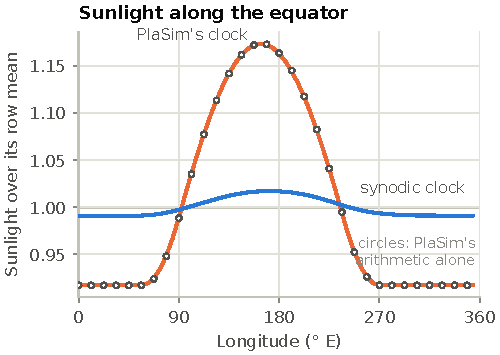
\includegraphics[width=0.6\textwidth]{figures/fig_sun_clock.pdf}
\caption{Sunlight at the top of the air along the equator, by longitude, over its row mean. Under PlaSim's
own Sun clock (run \code{A28\_dim5}, years 15--24) the Sun sweeps 392.5\textdegree\ each model day and skips
back 32.5\textdegree, leaving 270--57\textdegree~E 8.3\% short and the far side up to 17\% over; the circles
rebuild that pattern from PlaSim's solar-position arithmetic alone. Under the synodic clock
(\code{A28\_dim5\_sun\_test}) the row varies only by the 0.991--1.017 that 12.1 lunar days in a model year
give.}
\label{fig:sunclock}
\end{figure}

\textbf{Defects of the adaptation.} The adaptation made defects of its own, found some by checks of the
kinds set out under Verification and some in the course of the work. The GCM runner first extended the solar
spectrum past its 2.73~\textmu m end at its last value, an invented infrared tail that put 86\% of the
sunlight in the near infrared and warmed the first run past 320~K.\claim{H28} The first electrified build
discharged once per 6~s step, after all the step's charging, so the field stood a median 3.2 times breakdown
at a step's first discharge, which removed a median 150~C. Its fall-speed scaling multiplied memory the
scheme had left unset, and an OpenMP directive made private a variable the threads shared, both caught when
results changed with the thread count; and the first lunar gravity patch scaled the NSSL fall speeds and
missed the ventilation tied to them, so lunar rain evaporated 1.3--1.5 times too fast for its size until a
code review found it.\claim{H29} The sky model's 114 production channels averaged optical depth over windows
and opaque lines and absorbed 58\% too much sunlight above 500~nm with the Sun overhead, which had made
PlaSim look short of its calibration; the curved-air ledger's first channels, bisected on the whole column
alone, put near-infrared sunlight too high, 19.0 against 10.7~W\,m$^{-2}$ at 66--85~km, and the first two
20-year GCM tests of the curved air ran on those terms.\claim{H30} The first terrain build placed its forcing
by a corner column standing 2.9~km up. CM1's starting soundings held the GCM's top-level vapour constant above
the GCM's 130~km top, 6--15 times saturated over ice at 140--150~km in the 45\textdegree\,N rings, and the
45\textdegree\,N twilight pair ran its two halves on builds compiled at different optimisation
levels.\claim{H31} The last two remain in the runs made before they were found.

\textbf{What a slice of the GCM lacks.} Running CM1 inside the GCM's climate adds a structural limit to
the inherited ones. A ring of columns along a latitude circle misses the transport across the circle, a
box misses any day--night circulation larger than itself, and stock CM1 needs three things added: a lunar
Sun, forcing above its boundary layer and nudging that follows terrain. Two of these absences showed in
runs. The first box, forced with the advection along the rings alone, rained in the mornings and stayed
clear and hot in the afternoons until it was stopped at day 47, and at 45\textdegree\,N the missing
transport across the circle accounts for about a third of CM1's warm offset from the GCM.\claim{H32} The
forcing methods that answer these limits borrow from the GCM whatever the slice lacks, and so inherit the
GCM's remaining Earth.

\begin{table}[p]
\caption{The inventory of hidden Earth on the paths the lunar runs use, at Terluna commit 186b294. Form: a
constant, a unit of time, geometry, a fit or simplification used beyond its range (Fit), or a defect. State: a
general repair; a general method with a lunar table; a calibration to the lunar design case; a setting of
the lunar scenario; a capability added; a bound; avoided by configuration; bypassed; mitigated; or open.
Opt-in repairs are off in the design case.}
\label{tab:inventory}
\footnotesize
\setlength{\tabcolsep}{4pt}
\renewcommand{\arraystretch}{1.08}
\begin{tabularx}{\textwidth}{@{}>{\raggedright\arraybackslash}p{0.15\textwidth}LL>{\raggedright\arraybackslash}p{0.085\textwidth}>{\raggedright\arraybackslash}p{0.125\textwidth}@{}}
\toprule
Part & Earth in the code & On the Moon & Form & State \\
\midrule
\multicolumn{5}{@{}l}{\textit{ExoPlaSim 3.4.2 (PlaSim)}} \\
Sun clock & Restarts each model day & Skips back 32.5\textdegree\ a day & Defect & General \\
Orbit default & Earth's orbit for 1~AD & Tilt 23.7\textdegree\ for 1.54\textdegree & Defect & General \\
Calendar & 360-day year of 17,280 steps & Output slips 120 steps a year & Time & General \\
Convective cover & Rain per model day & Cover $+0.42$ & Time & General \\
Cloud water & CCM3 height scale in metres & Cloud above 20~km nearly dry & Constant & General \\
Slant path & Horizon factor 35 & 13.5 for water, 7.1 for air & Geometry & Method, lunar table \\
Columns & Flat, lit with the Sun up & Miss a net 5.8~W\,m$^{-2}$ loss & Geometry & Method, lunar table \\
Shortwave gases & Omit CO$_2$ and O$_2$ & Their share taken by water & Fit & Calibration \\
Rayleigh, continuum & 5772~K normalisation; continuum 0.024 & First design run past 310~K & Fit & Calibration \\
Water absorptivity & Lacis--Hansen, Earth's paths & Air 7.7--8.2 points short & Fit & Calibration \\
Longwave by height & Sasamori's absorptivities & Lowest layers overcooled 10--12~W\,m$^{-2}$ & Fit & Calibration, opt-in \\
Cloud phase & Liquid optics for all cloud & Ice cloud at 165--204~K & Fit & General, opt-in \\
Saturation & Over liquid; Earth's top levels & Cloud at 136--149\% of ice saturation & Fit & Open \\
Lowest level & Probably the spectral transform & Up to 20~K cold in 0.8\% of windows & Defect & Open, screened \\
Dynamics & Constant $g$, thin shell & $g$ 5.4\% lower at 48.6~km & Geometry & Open \\
\midrule
\multicolumn{5}{@{}l}{\textit{CM1 release 22}} \\
Gravity & 9.81 in four routines on the lunar paths; fall speeds & Fall speeds 2.3--6 times too fast & Constant & General \\
Rain size & Mean under 2.8~mm; breakup from 0.3~mm & Stable drops 2.46 times larger & Fit & Open \\
RRTMG gases & CO$_2$ by year; Earth's trace gases & Earth's air & Constant & Setting \\
RRTMG pressures & Tables from 1,053.63~hPa & Lowest 7.5~km extrapolated & Fit & Open \\
RRTMG ice & Optics to 140~\textmu m & Crash at day 6.45 & Fit & Mitigated \\
RRTMG Sun & Unfiltered spectrum & 5~W\,m$^{-2}$ of clear-air absorption & Constant & Open \\
Day & Earth's Sun and calendar; soil 1--16~cm & Thermal wave 0.6~m deep & Time & General (Sun); setting (soil) \\
Damping, mixing length & 300~s; 75~m & Earth's scales & Constant & General \\
Beta plane & Earth's rotation and radius & Earth's $\beta$ & Constant & Bypassed \\
Threads & Unlocated race & Runs on several threads part & Defect & Open \\
\midrule
\multicolumn{5}{@{}l}{\textit{WRF-ELEC, grafted into CM1}} \\
Gravity, ventilation & 9.8; fall speeds; ventilation & Fall speeds Earth's; scaled alone, rain evaporates 1.3--1.5 times too fast & Constant & General \\
Breakdown cap & 180~kV\,m$^{-1}$ & Binds below 36~km & Constant & General \\
Ground strike & $-7$\,\textdegree C level; stopping field 0.15 & Level 27--34~km up & Constant & Bound \\
Sub-step & 0.75~s for 500~m layers & 2~km layers, slow graupel & Constant & General \\
Flash reach & Logged above a charge threshold & Weak high flashes logged none & Constant & General (logging) \\
Conduction & None in clear air & Charge persists for weeks & Time & Capability \\
Charging, thresholds & Laboratory laws; 50~MV, 10~kV\,m$^{-1}$ & Polarity turns with the law & Fit & Open \\
\midrule
\multicolumn{5}{@{}l}{\textit{SWAN 41.51 and SWASH 12.01}} \\
Wind-input knee & 1~Hz & Similarity off by 5.44\% & Constant & General \\
Air density & 1.28~kg\,m$^{-3}$ & About 1.40~kg\,m$^{-3}$ & Constant & Setting \\
Breaker parameter & Read uninitialised with breaking off & Repeats differ by 2.5\% & Defect & Avoided \\
Other defaults & 2~s initial period; $g$ in ST6, XNL; Earth's radius, rotation & Earth's values & Constant & Avoided \\
Empirical laws & Wu, Komen, AGROW, breaker 0.73, breaking 0.6 and 0.3 & Uncalibrated & Fit & Open \\
\bottomrule
\end{tabularx}
\end{table}
